%!TEX root = ../main.tex

\chapter{Web Application Implementation}
\label{chp:webapp}

\paragraph{}
This chapter details the implementation of the SoundRise web application, a modern speech therapy tool utilizing CNN-based vowel recognition. We explore the system architecture, implementation, deployment, and testing processes, concluding with an analysis of performance and future development directions.

\section{System Architecture Overview}
\label{sec:architecture}

\paragraph{}
The SoundRise web application implements a modern client-server architecture designed specifically for speech therapy applications. The system's architecture emphasizes real-time processing capabilities and user experience, particularly focusing on providing immediate feedback for vowel pronunciation practice.

\paragraph{}
The frontend layer utilizes React.js to create a responsive and intuitive user interface, while the backend implements a Python-based REST API for audio processing and model inference. This separation of concerns allows for independent scaling and optimization of each component, ensuring optimal performance under varying load conditions.

\paragraph{}
The system implements comprehensive error handling and monitoring capabilities to ensure reliable operation in clinical settings. Real-time data processing pipelines are optimized to minimize latency while maintaining high accuracy in vowel recognition tasks, making the system suitable for interactive speech therapy sessions.

\section{Backend API Implementation}
\label{sec:backend-api}

\paragraph{}
The backend API is a crucial component of the SoundRise web application, enabling real-time vowel recognition through a trained CNN model. This section details the implementation of the API, the structure of the trained model file, and instructions for starting the API.

\subsection{API Implementation}
\label{subsec:api-implementation}

\paragraph{}
The API is implemented using Flask, a lightweight web framework for Python. It provides endpoints for processing audio data, generating spectrograms, and predicting vowel sounds using the trained model. The following code snippet illustrates the core functionality of the API:

\begin{lstlisting}[language=Python, caption={Backend API Implementation}]
import os
import tensorflow as tf
import numpy as np
from tensorflow.keras.preprocessing.image import ImageDataGenerator
import matplotlib.pyplot as plt
import librosa
import librosa.display
import base64
from flask import Flask, request, jsonify
from flask_cors import CORS
import io
from PIL import Image
import time

app = Flask(__name__)
CORS(app)

def create_data_generator():
    test_datagen = ImageDataGenerator(rescale=1./255)
    test_generator = test_datagen.flow_from_directory(
        'test',
        target_size=(55, 240),
        batch_size=8,
        class_mode='categorical',
        shuffle=False,
        color_mode='grayscale'
    )
    return test_generator

def main():
    app.run(host='0.0.0.0', port=5000, debug=True)

if __name__ == "__main__":
    main()
\end{lstlisting}

\subsection{Trained Model Structure}
\label{subsec:model-structure}

\paragraph{}
The trained model, referred to as \texttt{best\_model}, is stored in the \texttt{analysis} directory. It is saved in two formats: \texttt{best\_model.keras} and \texttt{best\_model.h5}. The API loads the model from this directory to perform predictions. The directory structure is as follows:

\begin{verbatim}
analysis/
    ├── best_model.keras
    └── best_model.h5
\end{verbatim}

\subsection{Starting the API}
\label{subsec:starting-api}

\paragraph{}
To start the backend API, ensure that all dependencies are installed and the trained model files are in place. Follow these steps:

\begin{enumerate}
    \item \textbf{Install Dependencies}: Ensure that all required Python packages are installed. This can be done using \texttt{pip}:
    \begin{verbatim}
    pip install tensorflow numpy flask flask-cors librosa matplotlib pillow
    \end{verbatim}

    \item \textbf{Run the API}: Execute the Python script to start the Flask server:
    \begin{verbatim}
    python <script_name>.py
    \end{verbatim}
    Replace \texttt{<script\_name>} with the name of your Python file containing the API code.

    \item \textbf{Access the API}: The API will be accessible at \texttt{http://0.0.0.0:5000/api/test-model}. You can send POST requests to this endpoint with audio data for vowel recognition.
\end{enumerate}

\paragraph{}
This setup provides a comprehensive backend solution for real-time vowel recognition, leveraging the trained CNN model to deliver accurate predictions.

\section{User Interface Design}
\label{sec:interface-design}

\paragraph{}
The user interface follows a clean, minimalist design philosophy that prioritizes accessibility and ease of use. As shown in Figure \ref{fig:homepage}, the homepage presents a welcoming interface with the SoundRise logo and clear navigation options. The design emphasizes visual clarity and intuitive interaction patterns, making it accessible to users of all ages and technical abilities.

\begin{figure}[htbp]
    \centering
    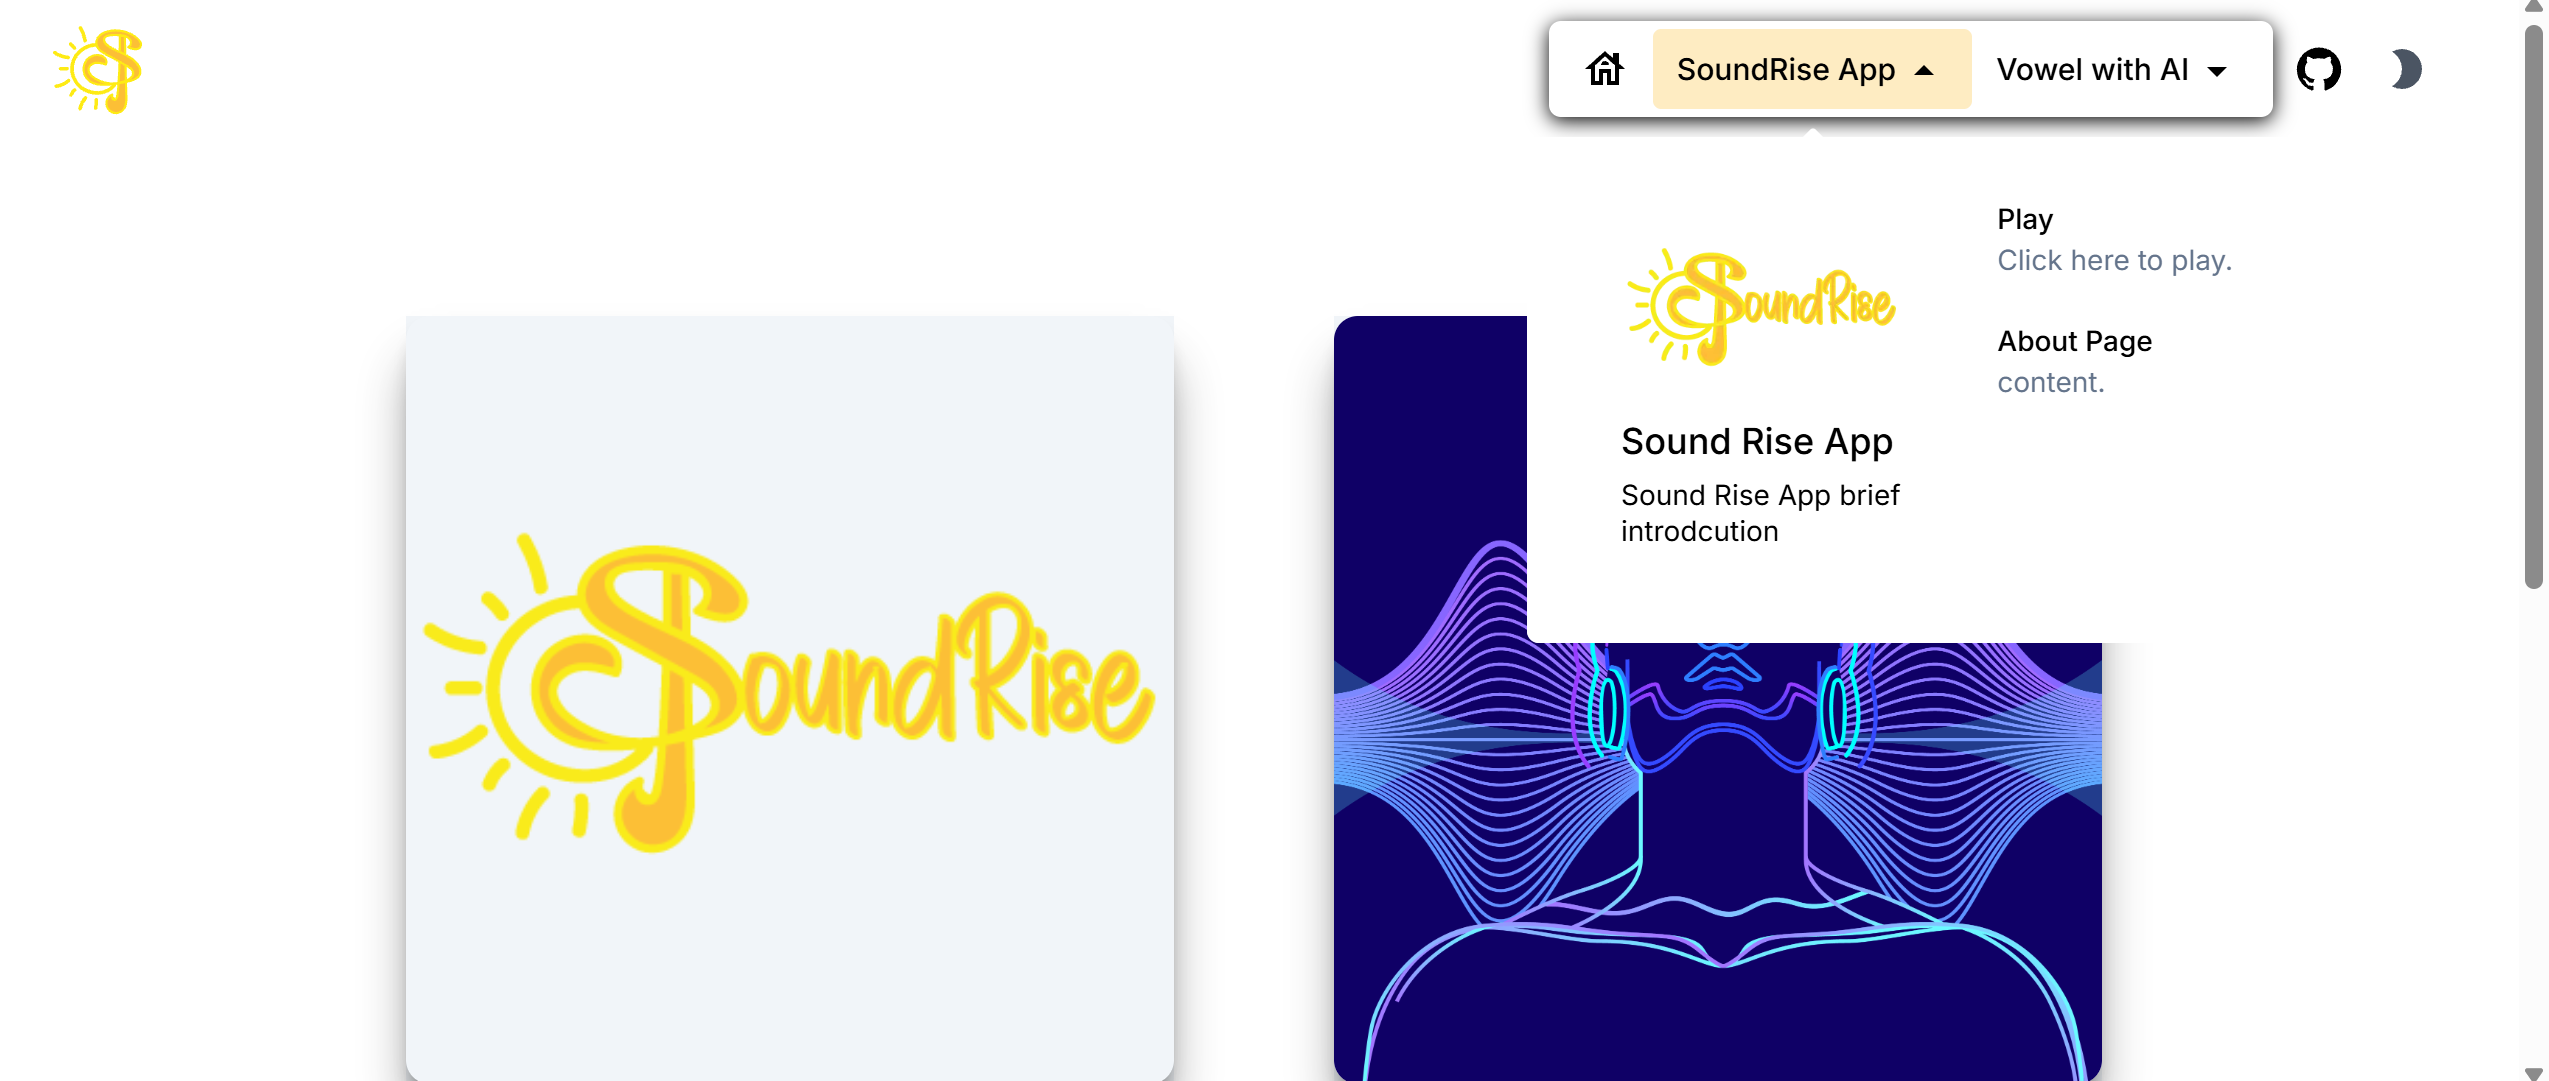
\includegraphics[width=0.8\textwidth]{res/images/webapp/homepage-1.png}
    \caption{SoundRise Homepage Interface}
    \label{fig:homepage}
\end{figure}

\paragraph{}
The application implements a comprehensive dark mode feature (Figure \ref{fig:dark_mode}) to accommodate different user preferences and environmental conditions. This feature not only enhances visual comfort but also reduces eye strain during extended practice sessions, particularly important for users who may require longer periods of practice.

\begin{figure}[htbp]
    \centering
    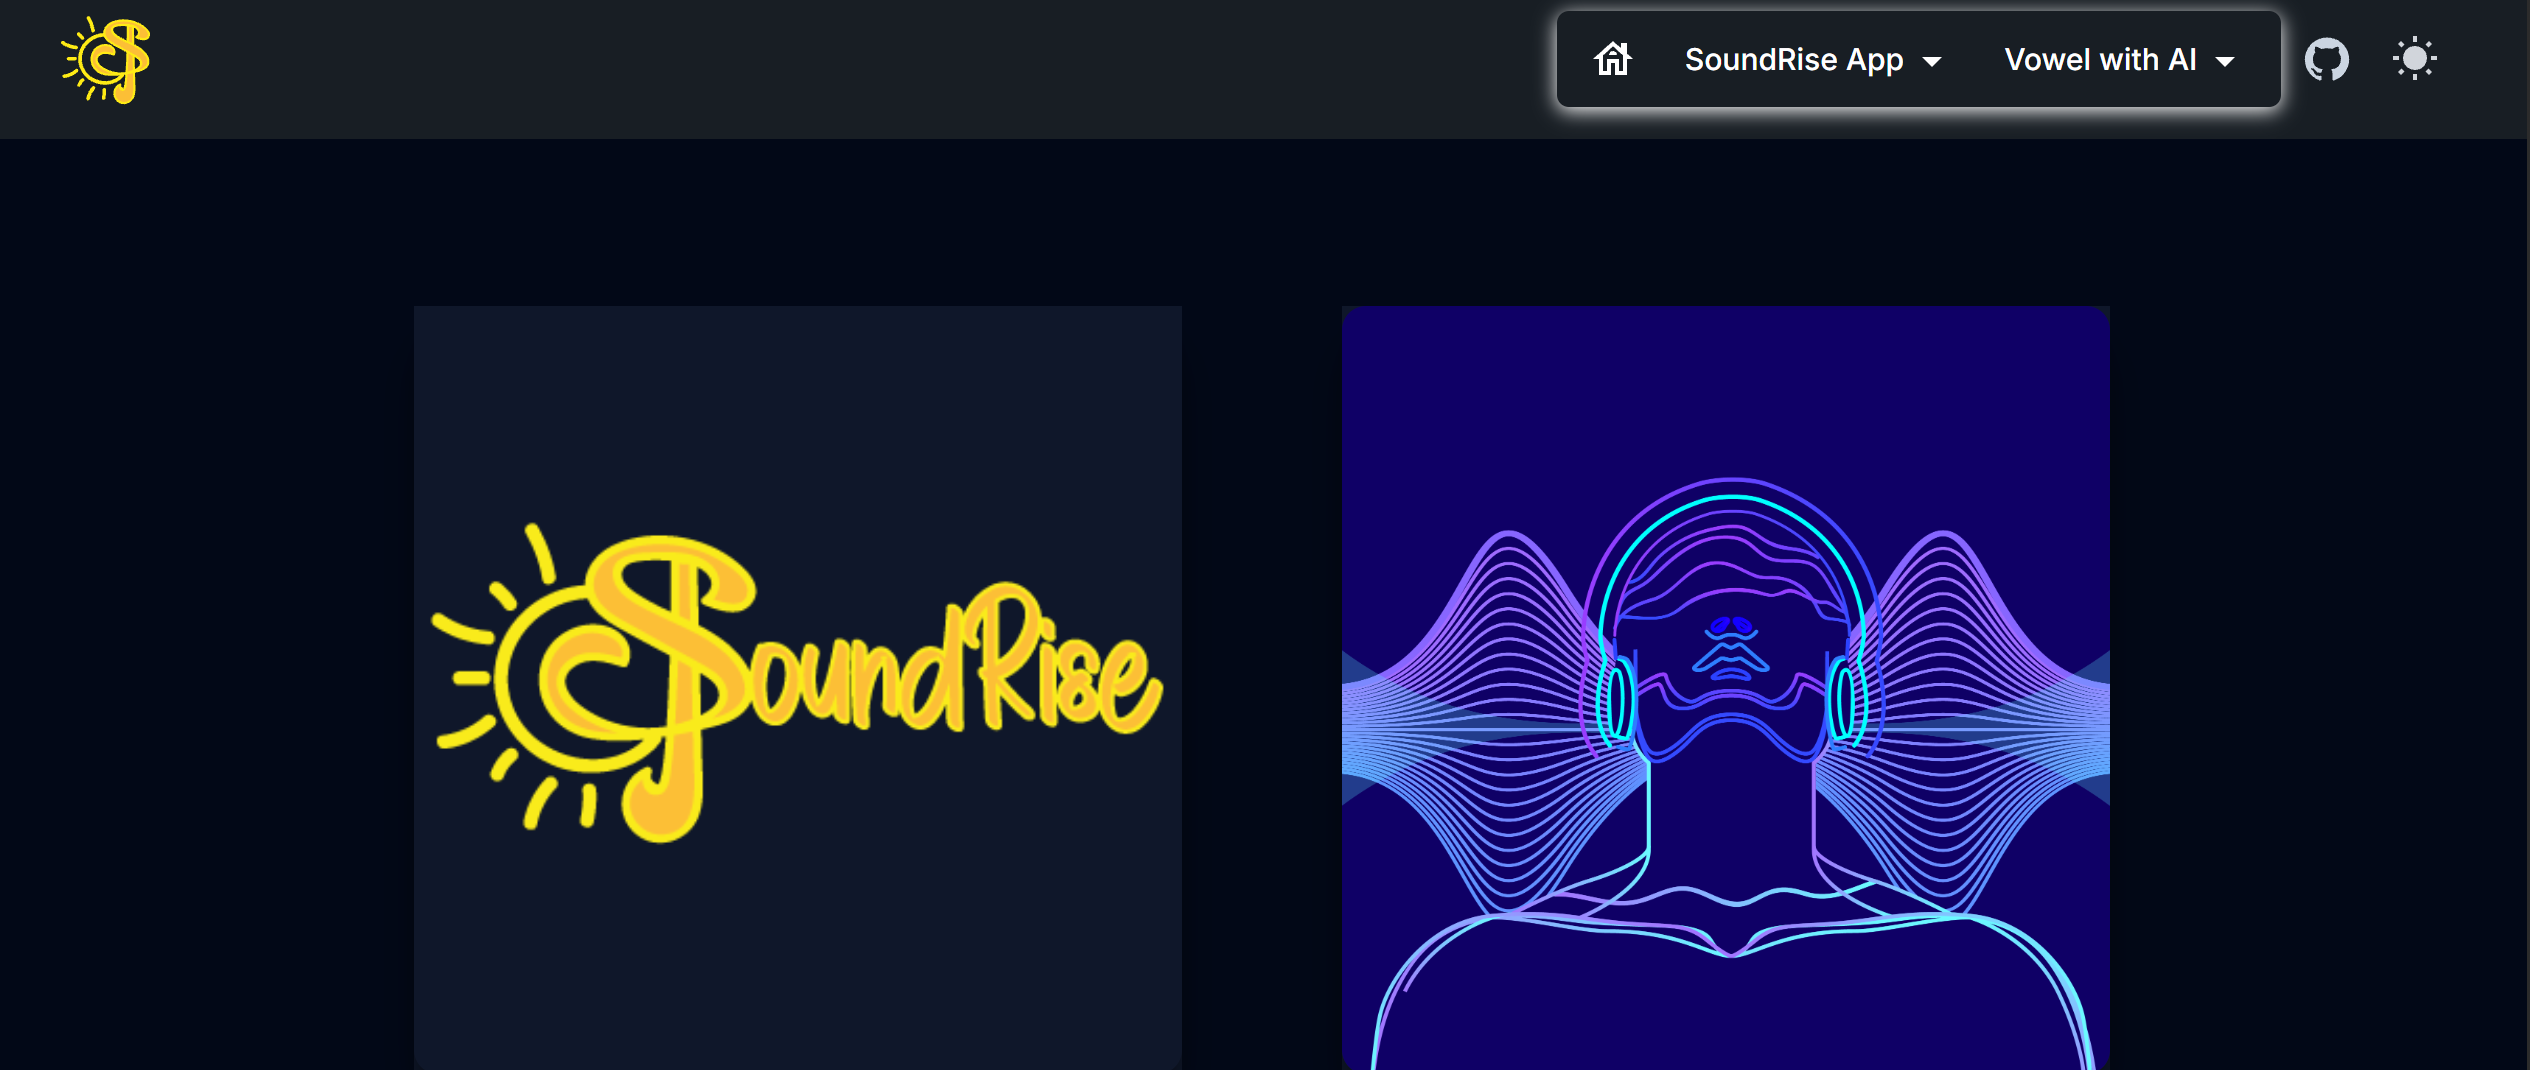
\includegraphics[width=0.8\textwidth]{res/images/webapp/homepage-darkMode.png}
    \caption{Dark Mode Interface}
    \label{fig:dark_mode}
\end{figure}

\paragraph{}
The header section (Figure \ref{fig:header}) provides clear navigation and system status information, including documentation access and user settings. This consistent header design maintains user orientation throughout the application while providing quick access to essential features and help resources.

\begin{figure}[htbp]
    \centering
    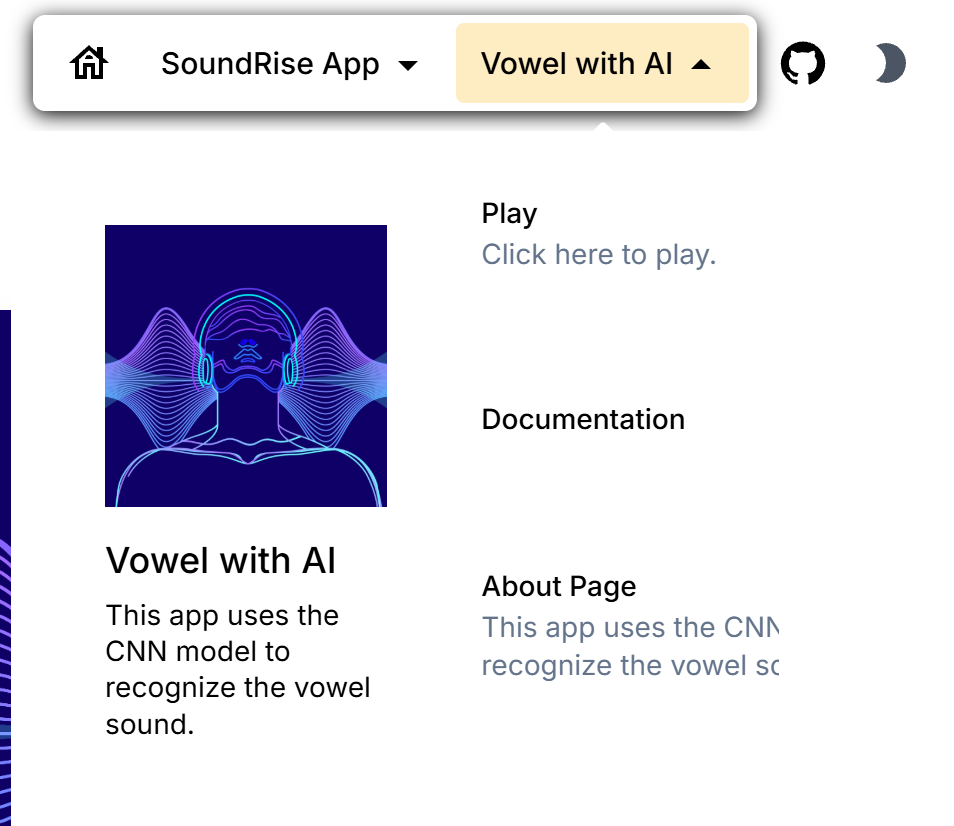
\includegraphics[width=0.8\textwidth]{res/images/webapp/homepage-header.png}
    \caption{Application Header with Navigation Elements}
    \label{fig:header}
\end{figure}

\section{Training Interface Implementation}
\label{sec:training-interface}

\paragraph{}
The training interface (Figure \ref{fig:interface_training}) represents the core functionality of the application, providing real-time feedback during vowel pronunciation practice. The interface combines audio recording controls with visual feedback mechanisms, creating an engaging and informative practice environment.

\begin{figure}[htbp]
    \centering
    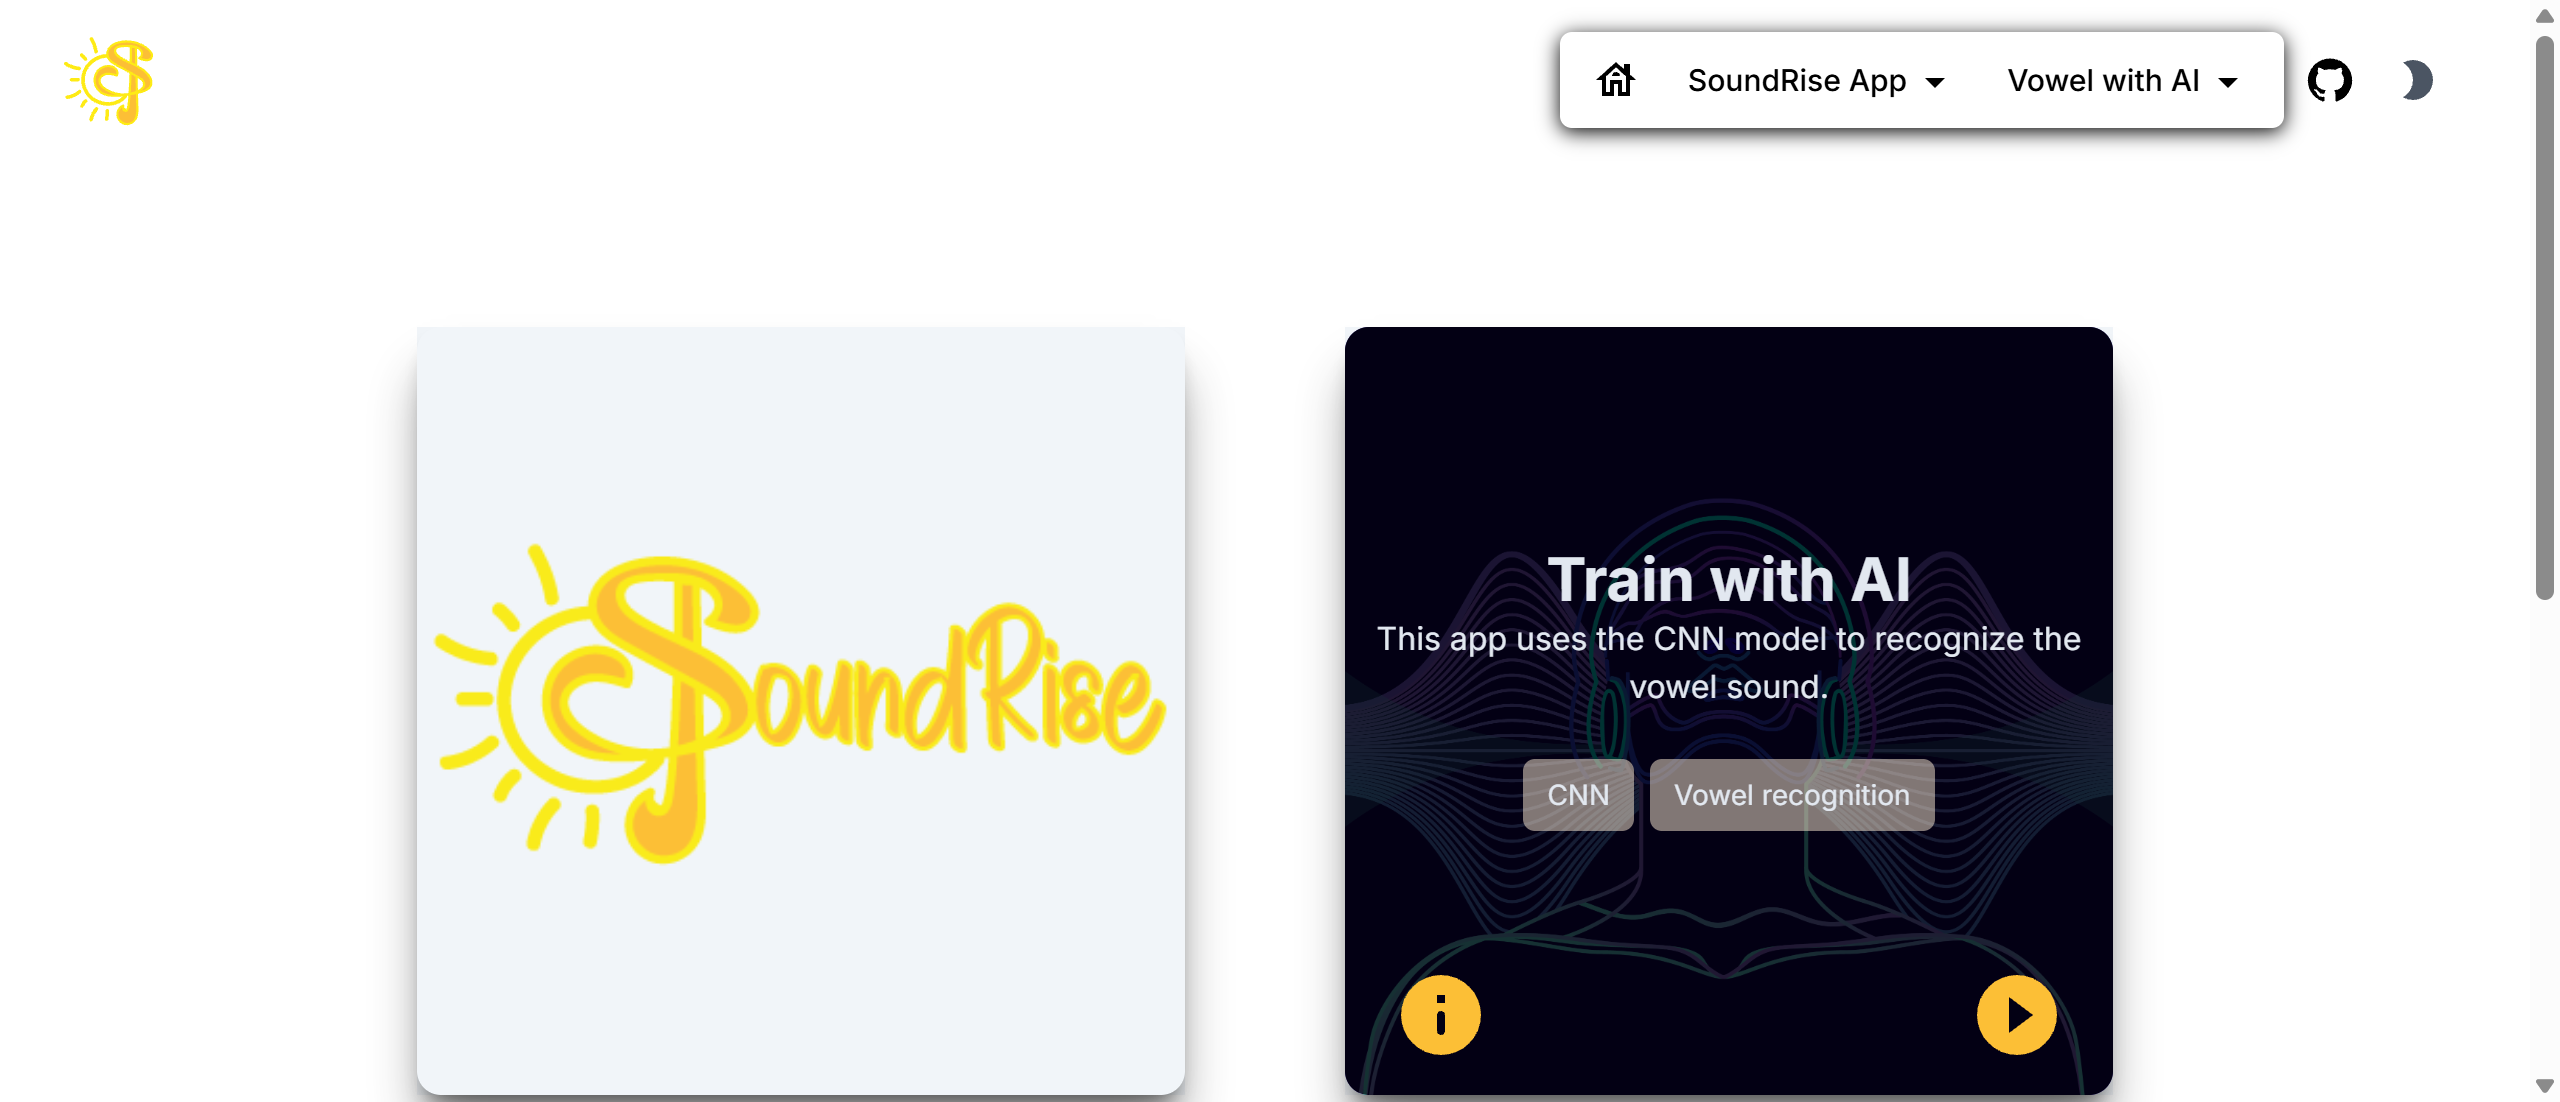
\includegraphics[width=0.8\textwidth]{res/images/webapp/interface.png}
    \caption{Main Training Interface}
    \label{fig:interface_training}
\end{figure}

\paragraph{}
The SoundRise information panel (Figure \ref{fig:info}) displays detailed metrics including pitch and intensity measurements, along with a comprehensive note grid for musical reference. This integration of musical elements helps users understand the relationship between pitch, intensity, and correct vowel pronunciation, providing multiple perspectives for improvement.

\begin{figure}[htbp]
    \centering
    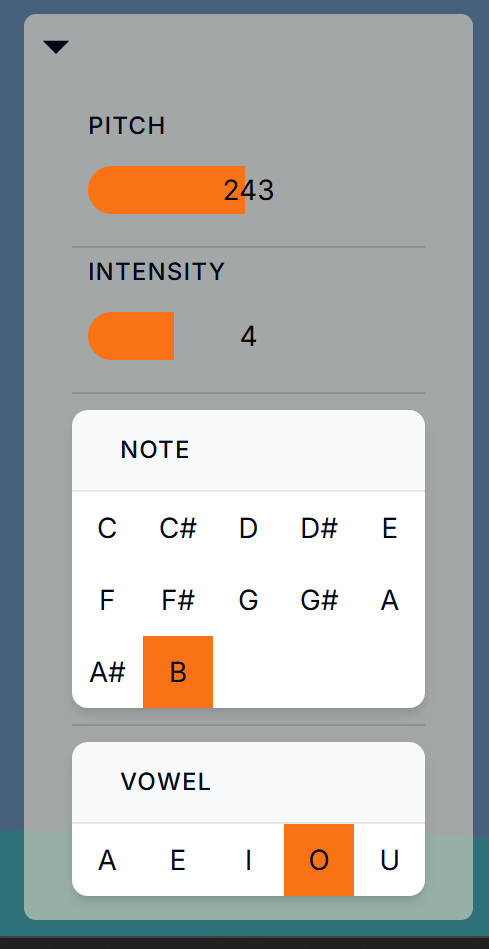
\includegraphics[width=0.4\textwidth]{res/images/webapp/soundRise-info.png}
    \caption{SoundRise Information Panel}
    \label{fig:info}
\end{figure}

\paragraph{}
The interactive feedback system (Figure \ref{fig:feedback}) uses emoticon-based visual cues to provide immediate, intuitive feedback on pronunciation accuracy. This gamification element helps maintain user engagement while providing clear indicators of performance, particularly beneficial for younger users or those new to speech therapy.

\begin{figure}[htbp]
    \centering
    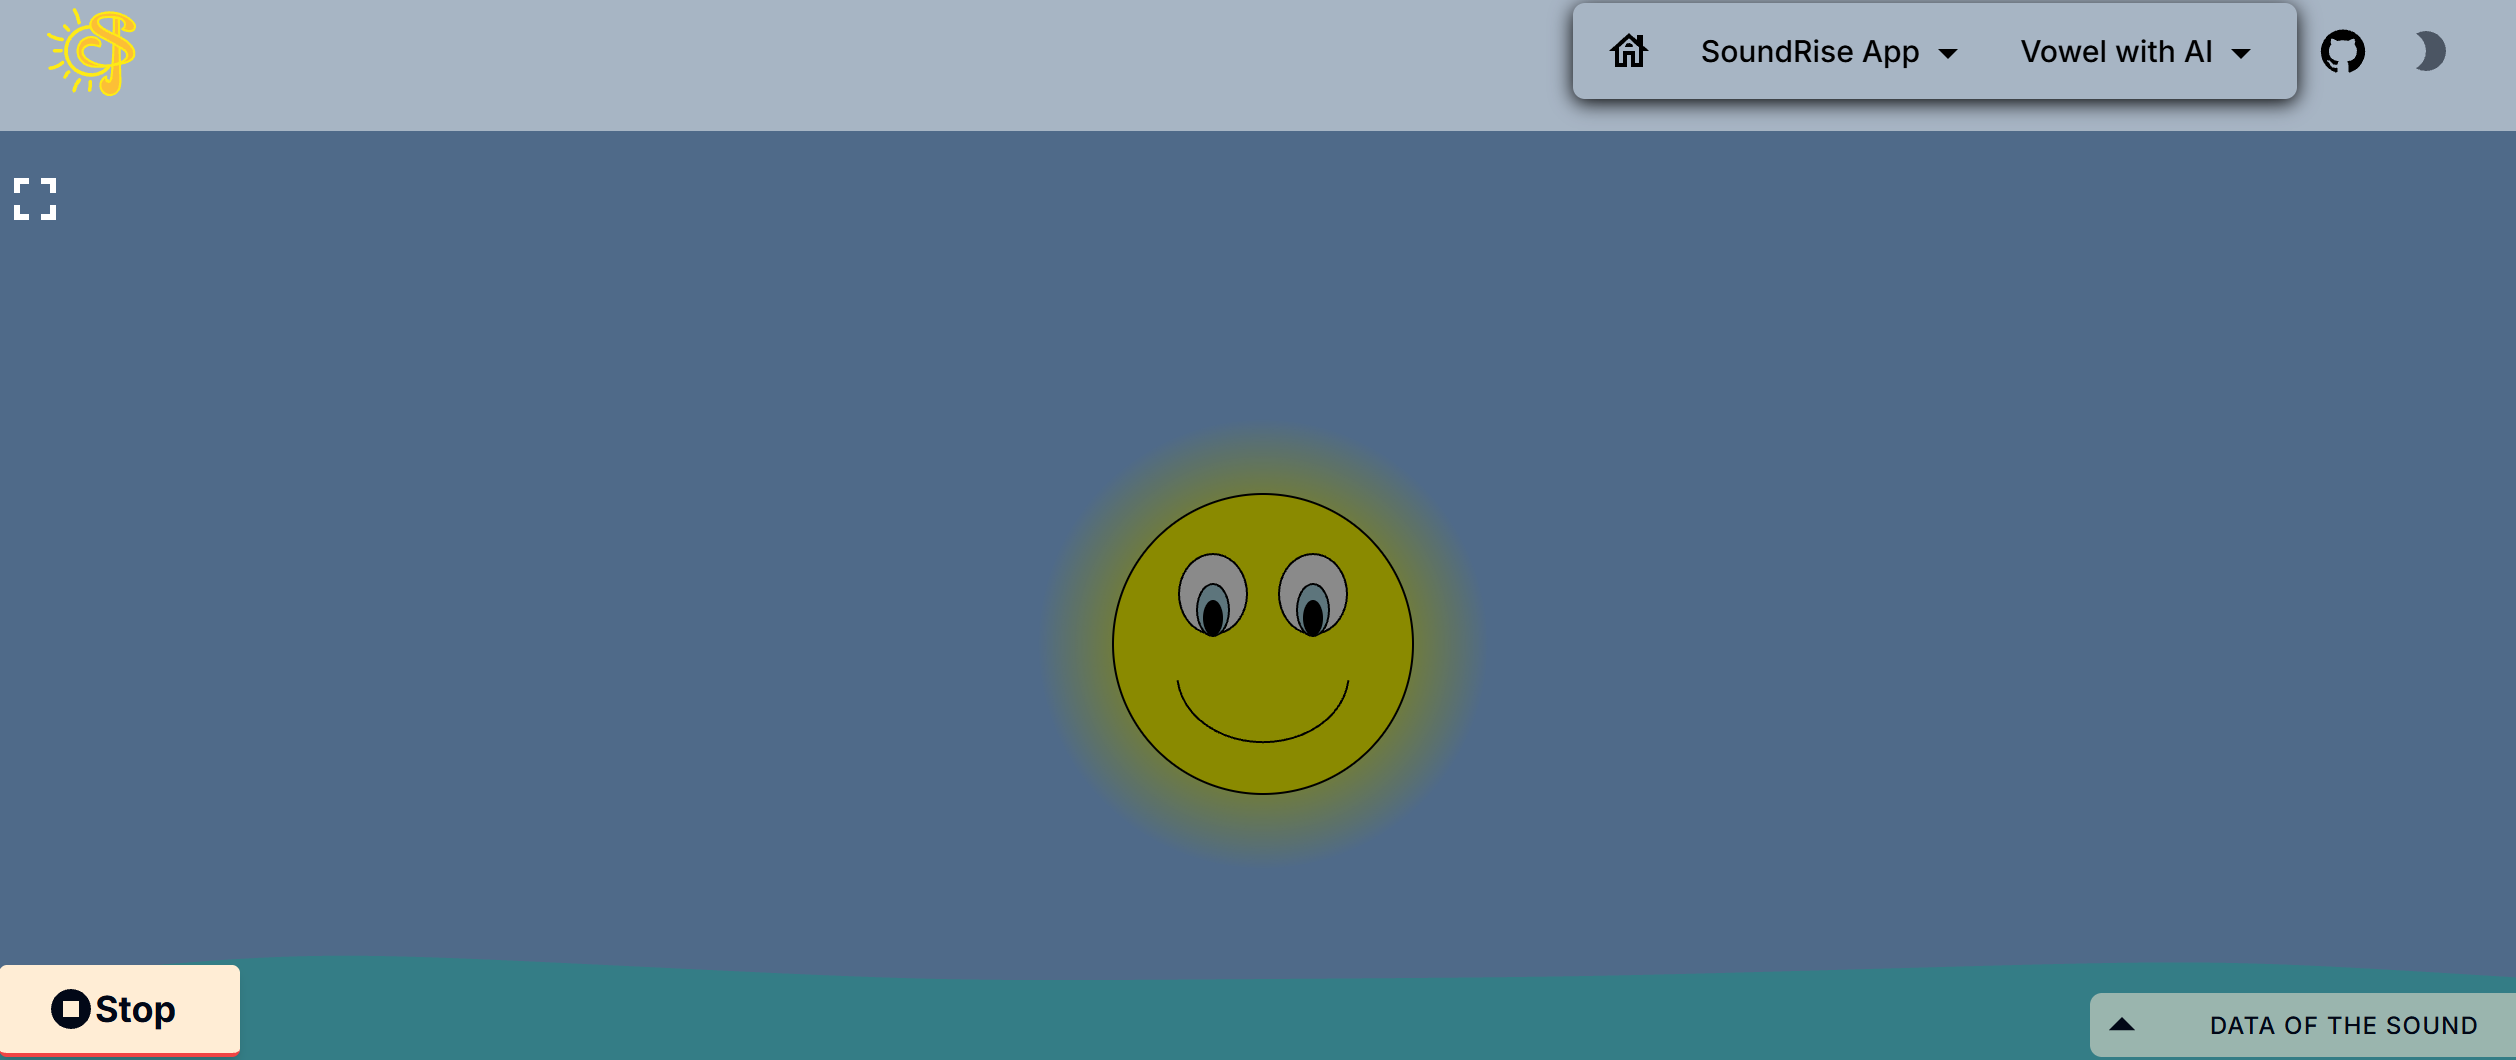
\includegraphics[width=0.4\textwidth]{res/images/webapp/soundRise-1.png}
    \caption{Interactive Feedback Display}
    \label{fig:feedback}
\end{figure}

\section{Results Visualization}
\label{sec:results-visualization}

\paragraph{}
The results interface (Figure \ref{fig:test_result}) provides comprehensive analysis of each pronunciation attempt. The visualization includes spectral analysis, confidence scores, and detailed feedback on pronunciation accuracy, presented in an accessible format that helps users understand their performance.

\begin{figure}[htbp]
    \centering
    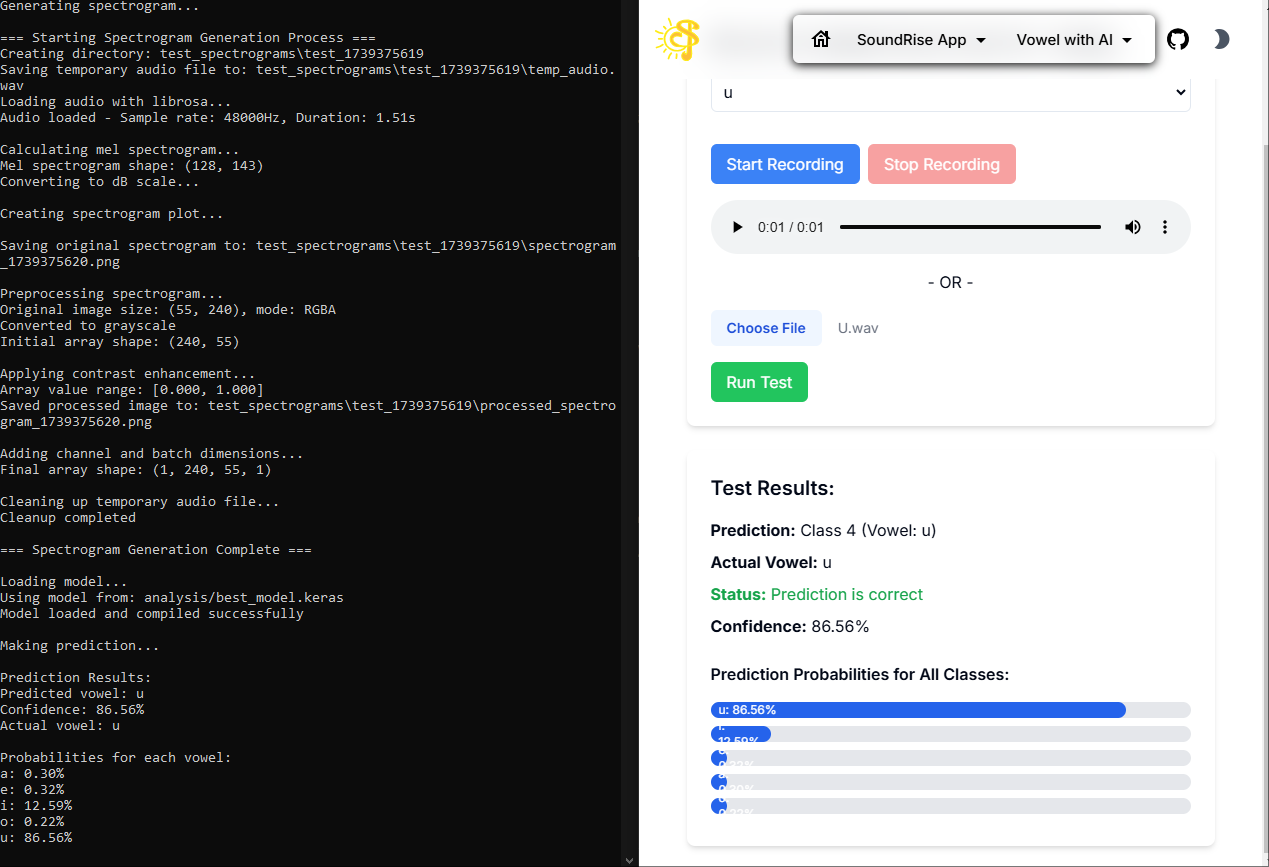
\includegraphics[width=0.8\textwidth]{res/images/webapp/testResult.png}
    \caption{Test Results Interface}
    \label{fig:test_result}
\end{figure}

\paragraph{}
The system implements a sophisticated visualization pipeline that processes real-time audio data and presents it in multiple formats. Users can view their pronunciation attempts through waveform displays, spectrogram visualizations, and numerical metrics, providing multiple perspectives on their performance.

\paragraph{}
Performance tracking features maintain detailed records of practice sessions and achievement metrics. The interface presents this data through intuitive visualizations that help users and therapists monitor progress over time, identify areas for improvement, and adjust practice strategies accordingly.

